\chapter{Caso di studio}
\section{OSGi}
La tecnologia OSGi è un insieme di specifiche che definiscono dei componenti
dinamici per l'ambiente Java. Queste specifiche, garantiscono lo sviluppo di
applicazioni composte da "moduli" i quali possono essere riutilizzati per
applicazioni future. Nel framework OSGi questi moduli prendono il nome di
\emph{bundle}. Similmente  alle applicazioni \emph{jar}, ogni bundle è composto
dai files contenti le classi ed i metodi specifici per la applicazione che
implementa. Quello che lo differenzia da un applicazione \emph{jar} è la
presenza al suo interno di metadati utili al framework OSGi per determinare
quali classi sono private ed utilizzabili solo all'interno dell'esecuzione del
modulo, da quelle che possono essere esposte e riutilizzate dagli altri moduli.
La possibilità del riutilizzo di questi moduli permette di
creare applicazioni di ridotta complessità che utilizzano le API di .
\subsection{Ciclo vitale dei bundle}
Data la modularità che questo framework offre, può capitare che dei bundle
richiedano di utilizzare delle API messe a disposizione da un bundle non ancora
presente nel sistema. Inoltre è necessario che questi errori vengano gestiti dal
framework in modo tale da non bloccare l'esecuzione delle applicazione.
Per questo motivo OSGi ha implementato vari stati in cui un bundle può trovarsi:
\begin{itemize}
        \item   \textit{Installed} Il bundle è stato installato nel sistema, ma
                non sono presenti alcune delle sue dipendenze.
        \item   \textit{Resolved} Il bundle è installato e le sue dipendenze
                presenti nel sistema.
        \item   \textit{Starting} Uno stadio temporaneo attraverso il quale il
                bundle passa prima di essere attivato.
        \item   \textit{Active} Il bundle è stato correttamente attivato e sta
                eseguendo le sue funzioni all'interno del sistema.
        \item   \textit{Stopping} Uno stadio temporaneo in cui il bundle passa
                prima di essere disattivato.
        \item   \textit{Uninstalled} Il bundle è stato rimosso dal container
                OSGi
\end{itemize}
\subsection{Registrazione del servizio}
La classificazione del tipo di classi che un bundle implementa, vine
interpretata dal framework OSGi grazie ai metadati aggiuntivi all'interno del
bundle stesso. È necessario quindi avere un registro nel quale if framework osgi
raggruppa tutti i metodi esposti e richiesti dai vari bundle in modo tale che 
attivando un nuovo bundle, questo registro venga aggiornato e sia possibile
determinare se altri bundle posso passare da disattivi ad attivi.
La soluzione a questo, è l'utilizzo di registri di servizio. Ogni bundle può
esporre dei metodi ed registrarli attraverso il service registry. In questo
modo, altri bundle possono accedere al service registry e utilizzare i metodi
listati nel registro. Un bundle quindi può registrare un servizio, può
utilizzare un servizio oppure può mettersi in attesa aspettando che un servizio
venga registrato o eliminato.
\begin{figure}[h]
\centering 
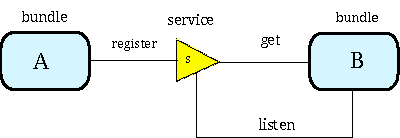
\includegraphics[width=10cm]{osgi_service}
\caption{OSGi services}
\label{}
\end{figure}
\subsection{Layer}
\begin{figure}[h]
\centering 
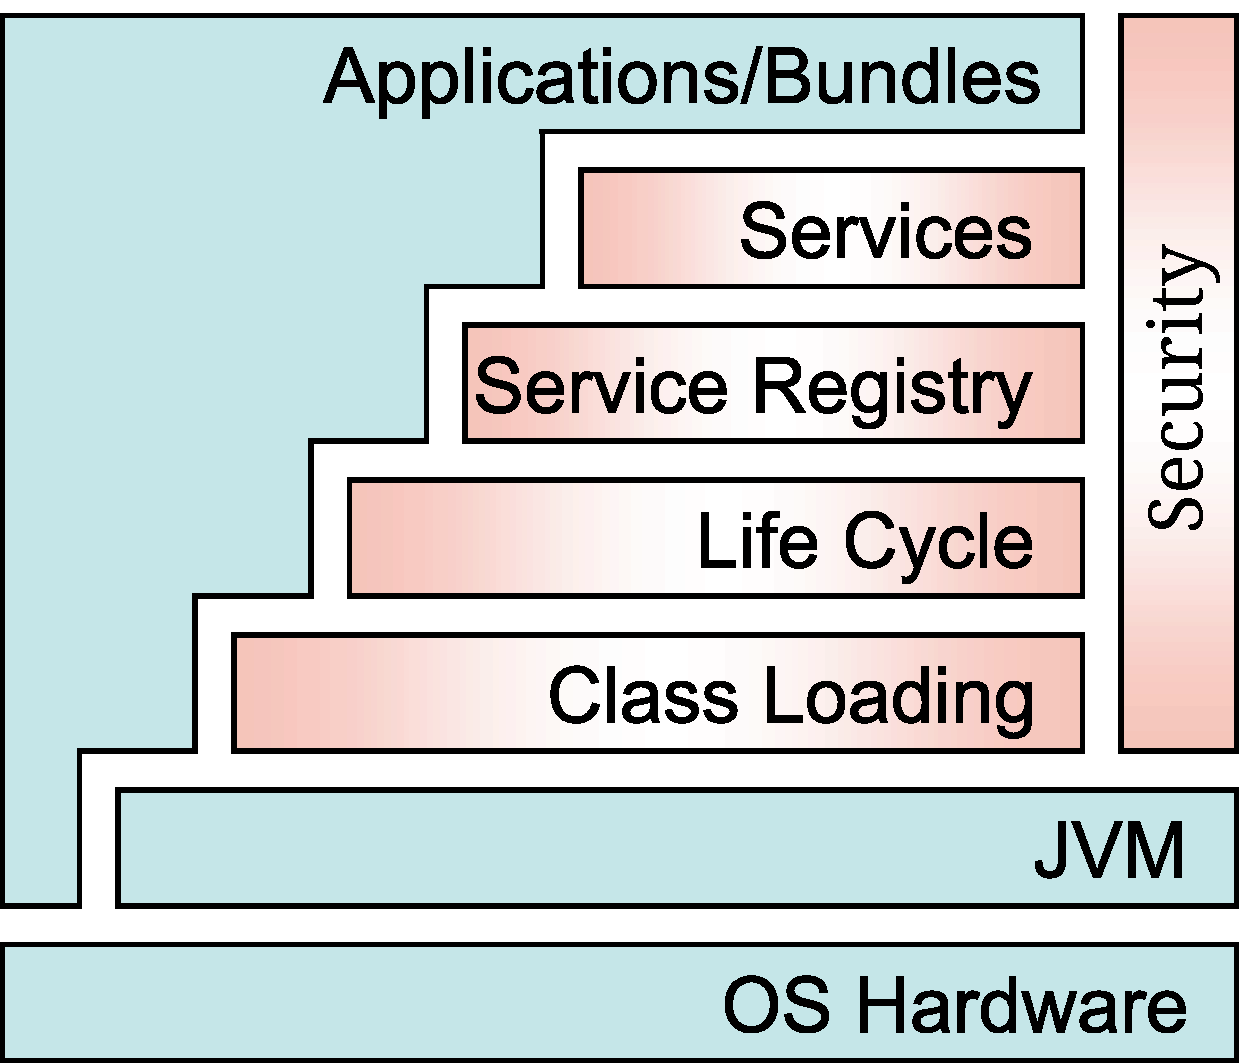
\includegraphics[width=10cm]{osgi}
\caption{Layer OSGi}
\label{}
\end{figure}



Il concetto alla base dello standard OSGi e modularità,


Utilizzando il modulo SX1301 in combinazione con il gateway prodotto da Eurotech
ReliaGATE 10-11, si è andato a sviluppare un software in grado di ricevere i
pacchetti inviati da dispositivi LoRa e inviarli ad un Broker Mqtt.

\subsection{SX1301}
Nella tabella \ref{tab:sx1301_spec} sono riportate le caratteristiche elettriche
massime del  chip SX1301. Il Chip, supporta tensioni di
alimentazione fino a 4V e  come e possibile osservare il range di temperatura in cui il
chip può operare è molto ampio, rendendolo ideali per applicazioni esterne ed
interne. 

\begin{table}[h]
\centering 
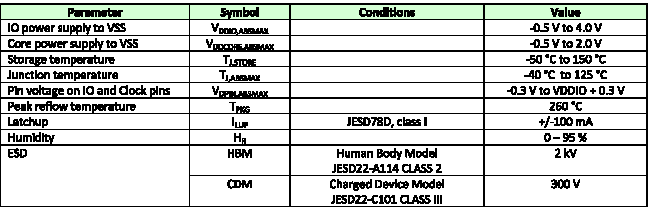
\includegraphics[width=16cm]{SX1301_table}
\caption{Caratteristiche elettriche SX1301}
\label{tab:sx1301_spec}
\end{table}
Utilizzando i valori nominali riportati nella tabella \ref{tab:sx1301_spec_1},
si hanno valori di corrente pari a 1[uA] in idle  e di 5[mA] in pieno
funzionamento.
\begin{table}[h]
\centering 
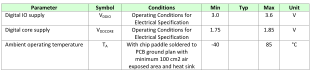
\includegraphics[width=16cm]{SX1301_table_1}
\caption{Caratteristiche elettriche SX1301}
\label{tab:sx1301_spec_1}
\end{table}
Il chip è equipaggiato con un connettore sma al quale è collegata una
antenna omindirezionale, ideata per la frequenza 868[MHz] con un guadagno pari a 3dB.
\subsection{ReliaGATE}
Il gateway a cui è collegato il modulo SX1301 è il ReliaGATE 10-11 prodotto da
Eurotech. Al suo interno troviamo un processore Texas Instruments TI AM335X Cortex-A8 
equipaggiato con 512MB di RAM e 4GB di storage eMMC. Il ReliaGATE offre una
vasta gamma di porte tra cui 232/485, 2CAN bus, 2 porte USB e 2 porte Ethernet,
inoltre ha connettività Bluetooth, WiFi e GPS. Al suo interno è installo
Everyware™ Software Framework (ESF), la versione commerciale del software Kura.
\begin{figure}[h]
\centering 
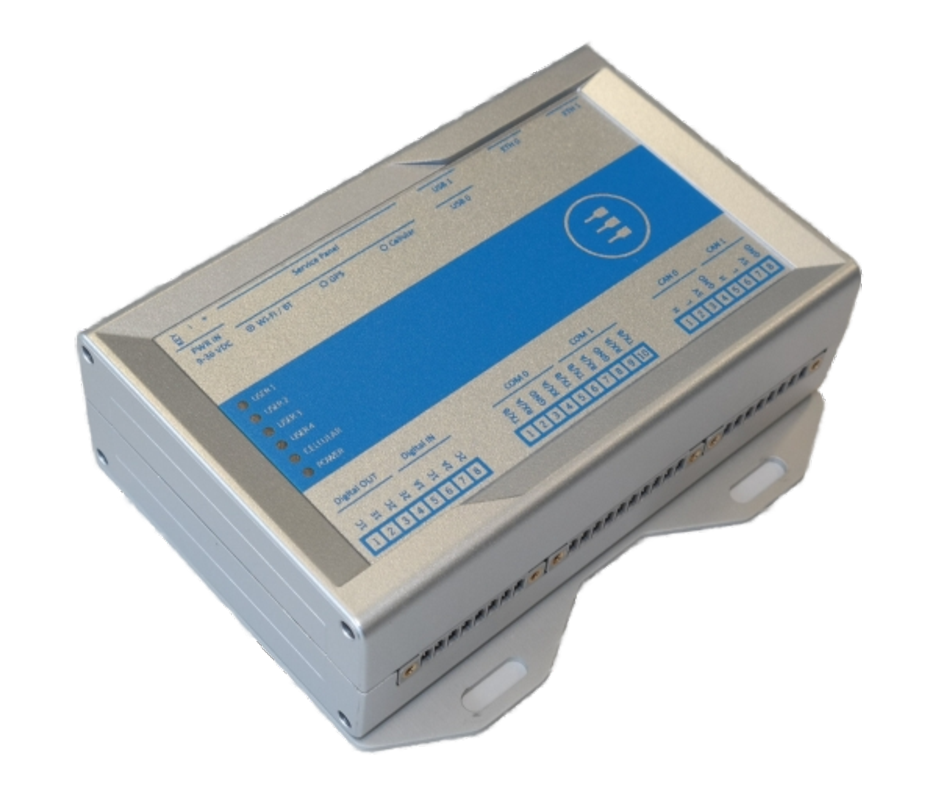
\includegraphics[width=11cm]{Reliagate_10_11}
\caption{Caratteristiche elettriche SX1301}
\label{fig:ReliaGATE}
\end{figure}


\subsection{Architettura del software}
Lo scopo di questa tesi era riuscire ad implementare dei moduli osgi,
installabili al interno del framework ESF, in grado di controllare il
comportamento del devices SX1301. In particolare utilizzando l'utility messa a
disposizione da Semtech per l'interfacciamento con il dispositivo denominata
packet forwarder, e l'utility LoRa Gateway Bridge , sotto licenza MIT,
sviluppata da brocaar \improvement{Aggiunger link}.

\begin{figure}[h]
\centering 
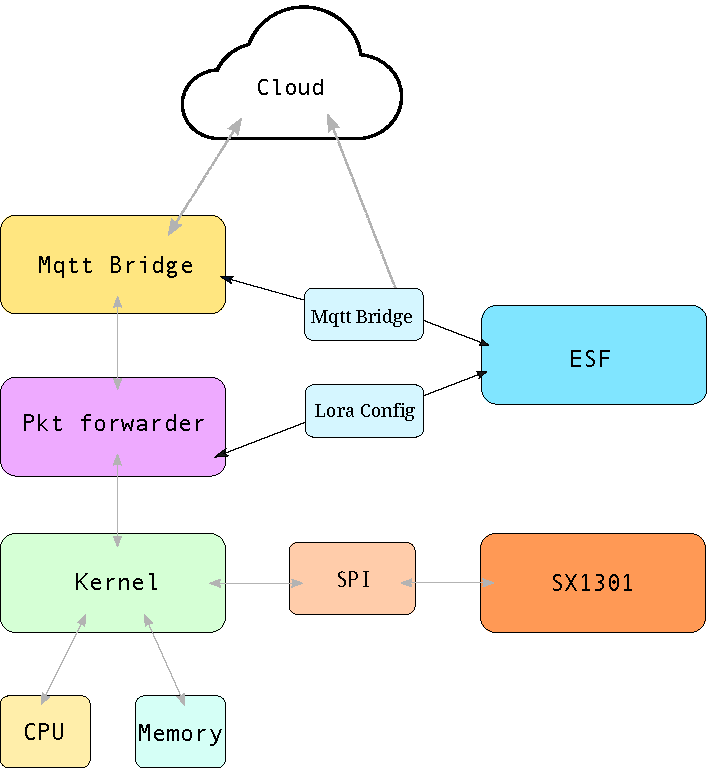
\includegraphics[width=11cm]{Application_layer}
\caption{Architettura del software}
\label{fig:Software_stack}
\end{figure}

\subsection{Semtech packet forwarder}
Il packet forwarder, è un software il quale riceve o invia pacchetti radio Lora ,
tramite una connessione SPI con il device SX1301. Nel caso di ricezione di un
pacchetto, l'applicativo incapsula i dati ricevuti in un formato IP/UDP, e li
ritrasmette nella rete internet/intranet. Per la sua configurazione viene
utilizzato un file Json nel quale trviamo tutte le varie opzioni di
configurazione per i moduli radio presenti al interno del chip.
\inputminted[mathescape, gobble=2, frame=lines, linenos=true
framesep=2mm, firstline=1,lastline=23]{json}{Code_Files/global_json.conf}
\inputminted[mathescape, gobble=2, frame=lines, linenos=true
framesep=2mm, firstline=173,lastline=184]{json}{Code_Files/global_json.conf}

\subsection{LoRa Gateway Bridge}
LoRa Gateway Bridge, è l'applicativo il quale riceve i vari pachetti UDP inviati
dal packet forwarder e li trasmette ad un Broker MQTT. Il software è scritto nel
linguaggio GO. Per renderlo interfacciabile con ESF, sono state apportate delle 
modifiche al codice, in particolare è stata aggiunta la possibilità di
specificare il publish e il subscribed topic, i quali erano hard-coded.

\subsection{ESF}
Everyware software framework, è la versione commerciale del software Kura
preinstallata nel ReliaGATE 10-11. ESF si pone l'obiettivo di offrire un
container Java/OSGi per le applicazioni M2M. Gli applicativi installati in ESF
sono sviluppati come OSGi Declarative Service, dando la possibilità di
configurare i vari applicativi del gateway tramite una semplice interfaccia web.

\begin{figure}[h]
\centering 
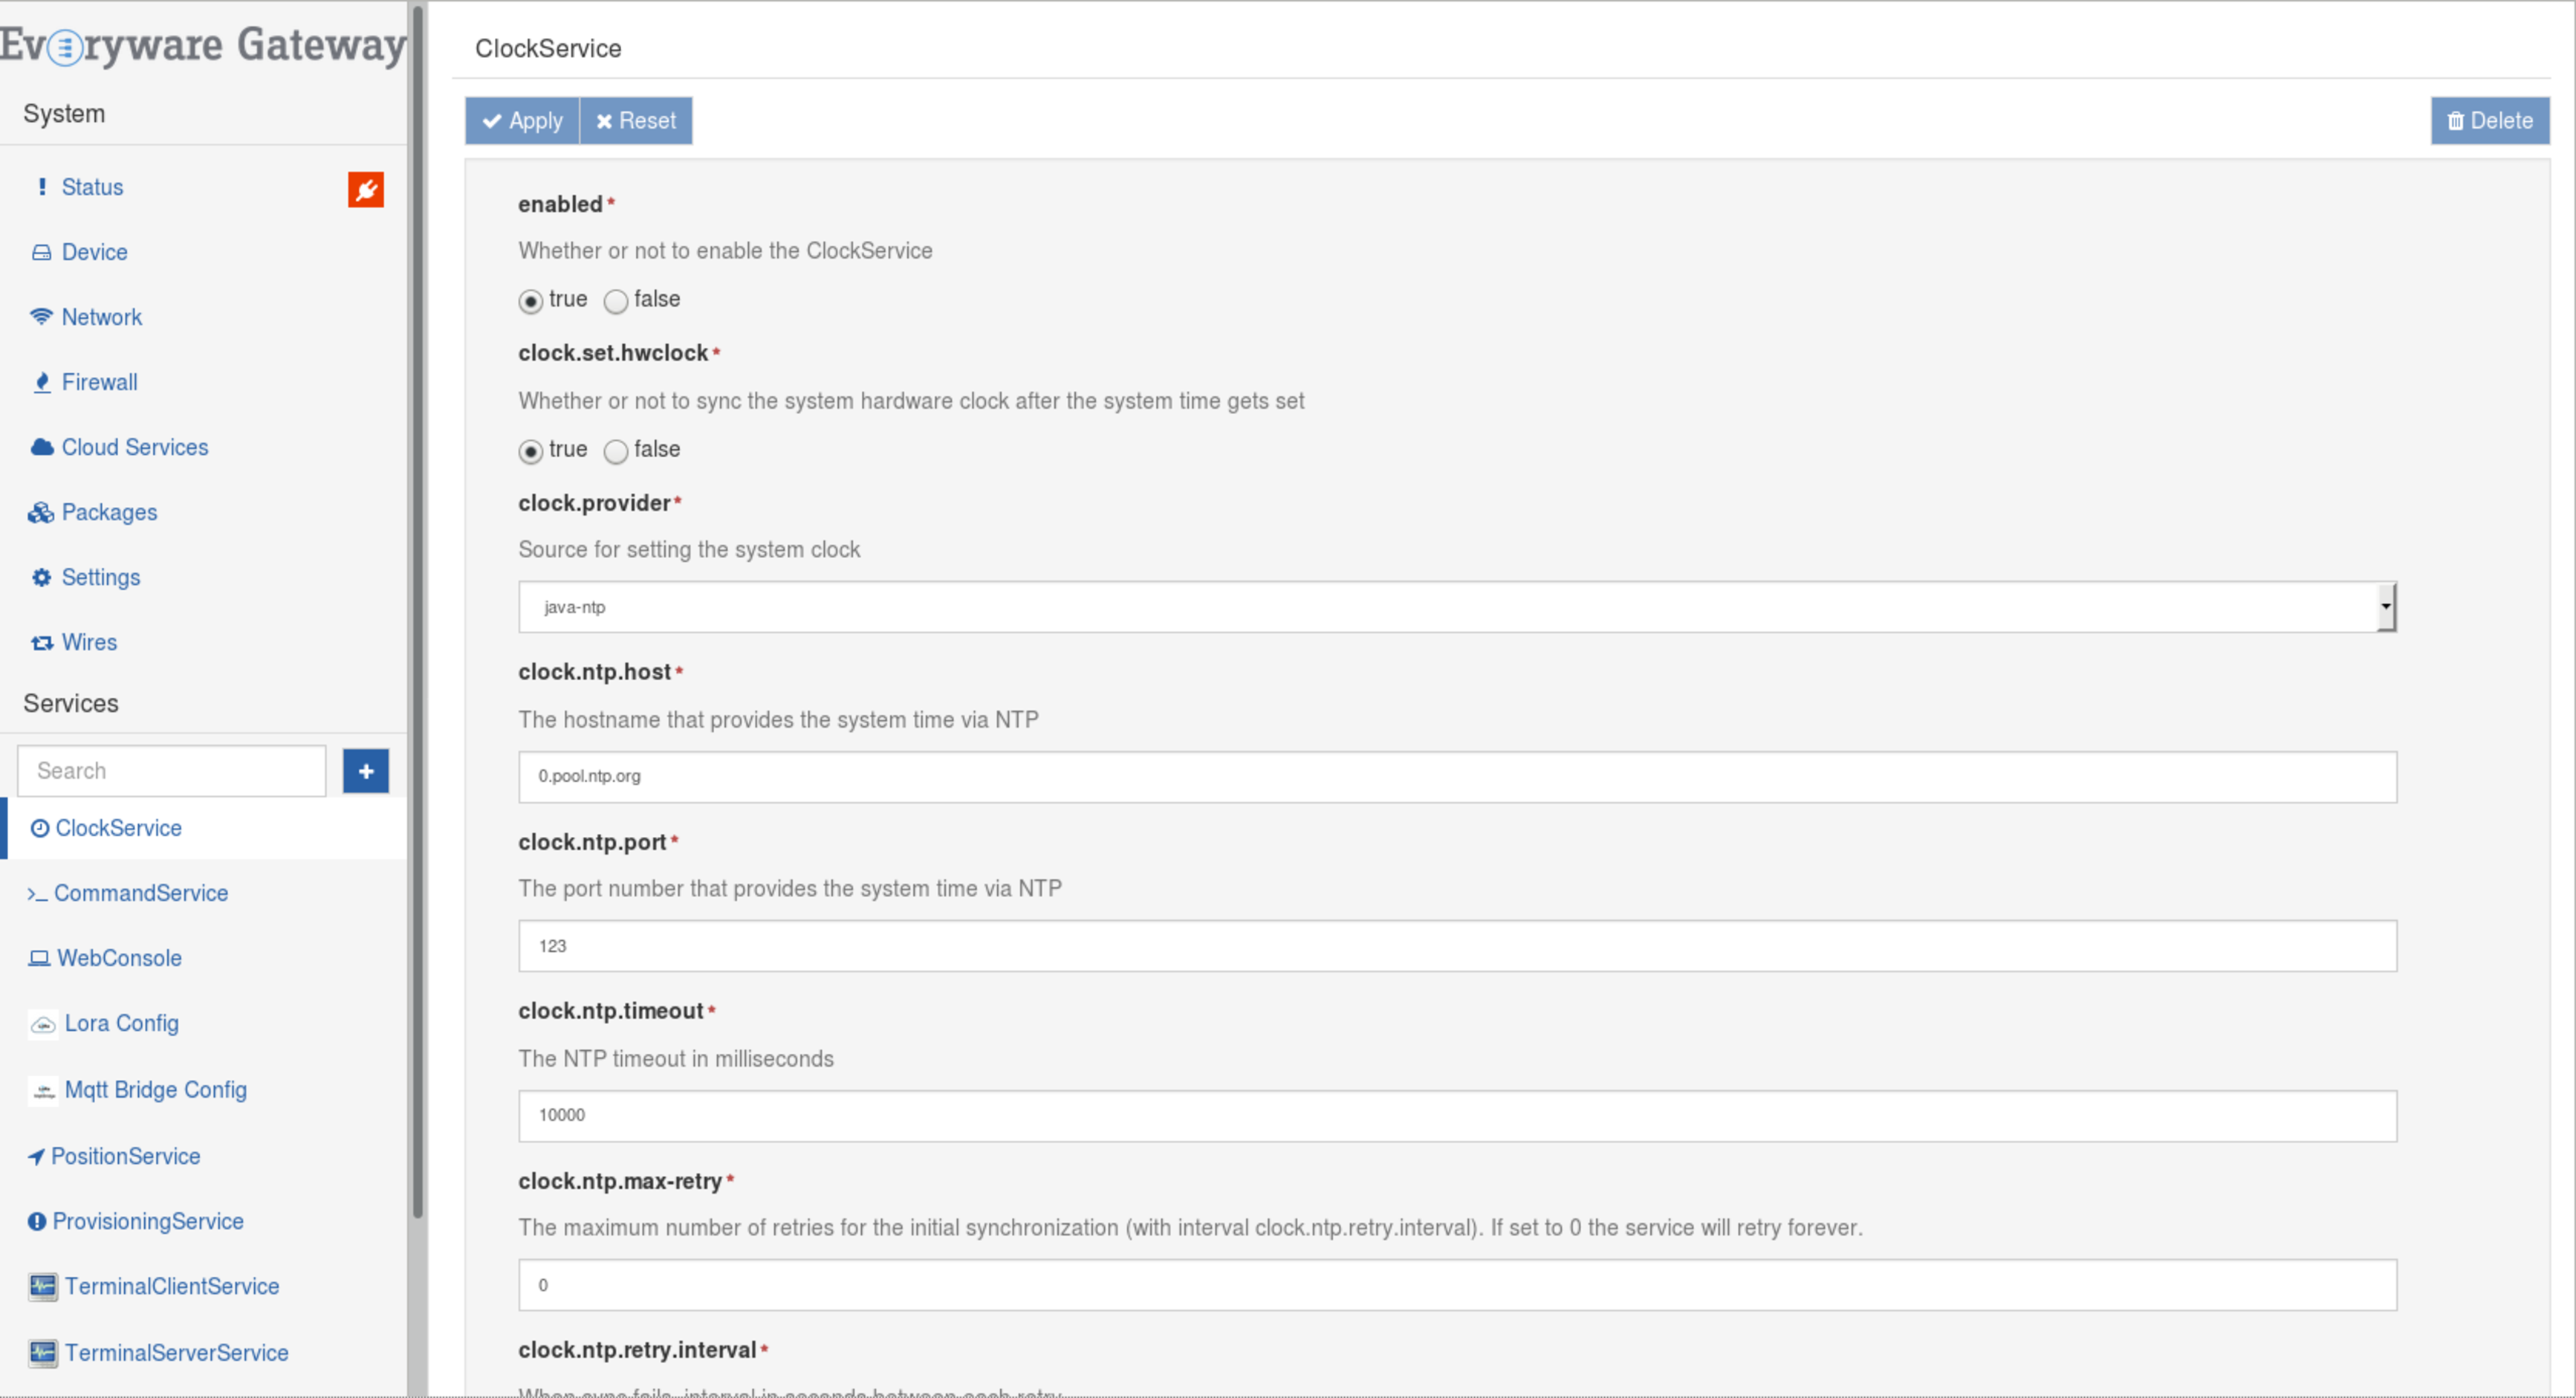
\includegraphics[width=16cm]{ESF.png}
\caption{Architettura del software}
\label{fig:Software_stack}
\end{figure}

\subsection{Realizzazione}
Per gestire i due software preinstallati si è optato per la creazione di due
applicativi osgi distinti.
Il primo applicativo chiamato Lora Config si pone il compito di leggere ed
interpretare il file di configurazione utilizzato dal programma \emph{Packet
Forwarder}, per poi andare ad esporre i punti principali al utente finale.
La libreria utilizzata per manipolare i file di tipo Json è 

\mint{Java}|import com.eclipsesource.json|

Tramite la quale vengono riempiti i campi della classe LoraSettings. Il file
Json, come detto precedentemente è composto da due parti. Nella prima parte
troviamo tutte le impostazioni per la configurazione del SX1301, nella seconda
parte sono presenti le impostazioni per il forward dei pacchetti. Per questa
ragione due classi diverse sono state create, SX1301Configuration e
GatewayConfiguration, accessibili tramite la classe LoraSettings.

\begin{minted}[linenos=true, numbersep=5pt, gobble=2, frame=lines, %
framesep=2mm]{java}
    public class LoraSettings {
            public static final String KEY_GATEWAY_CONFIG = "gateway_conf";
            public static final String KEY_SX1301 = "SX1301_conf";
            private SX1301Configuration sx1301Conf;
            private GatewayConfiguration gatewayConf;
        }
\end{minted}

Per applicare le modifiche eseguite alla configurazione, è necessario che
l'applicativo sia riavviato. Per eseguire questa operazione, si è scelto di
utilizzare la libreria 
\mint{Java}|import com.apache.commons.exec|
la quale fornisce delle \emph{API} per chiamare processi esterni, in particolare
si è scelto di utilizzare l'utility di sistema \emph{pkill} per terminare il
processo del pkt forwarder.
\begin{minted}[linenos=true, numbersep=5pt, gobble=2, frame=lines, %
framesep=2mm]{java}
          public void startPktForwarder() {
                DefaultExecutor pktExecutor = new DefaultExecutor();
                CommandLine pktCmdLine = new CommandLine(KEY_PKT_BIN);
                pktCmdLine.addArgument("start");
                pktExecutor.setExitValue(0);
                try {

                    pktExecutor.execute(pktCmdLine);
                    s_logger.info("start PKT");
                } catch (Exception e) {
                    s_logger.warn("Coulden't start pkt forwarder");
                }
            }

            public void stopPktForwarder() {
                DefaultExecutor pktExecutor = new DefaultExecutor();
                CommandLine pktCmdLine = new CommandLine("pkill");
                pktCmdLine.addArgument("basic_pkt_fwd");
                pktExecutor.setExitValue(0);
                try {

                    pktExecutor.execute(pktCmdLine);
                    s_logger.info("Stop PKT");
                } catch (Exception e) {
                    s_logger.warn("Coulden't stop pkt forwarder");
                }
        }

\end{minted}

\begin{figure}[h]
\centering 
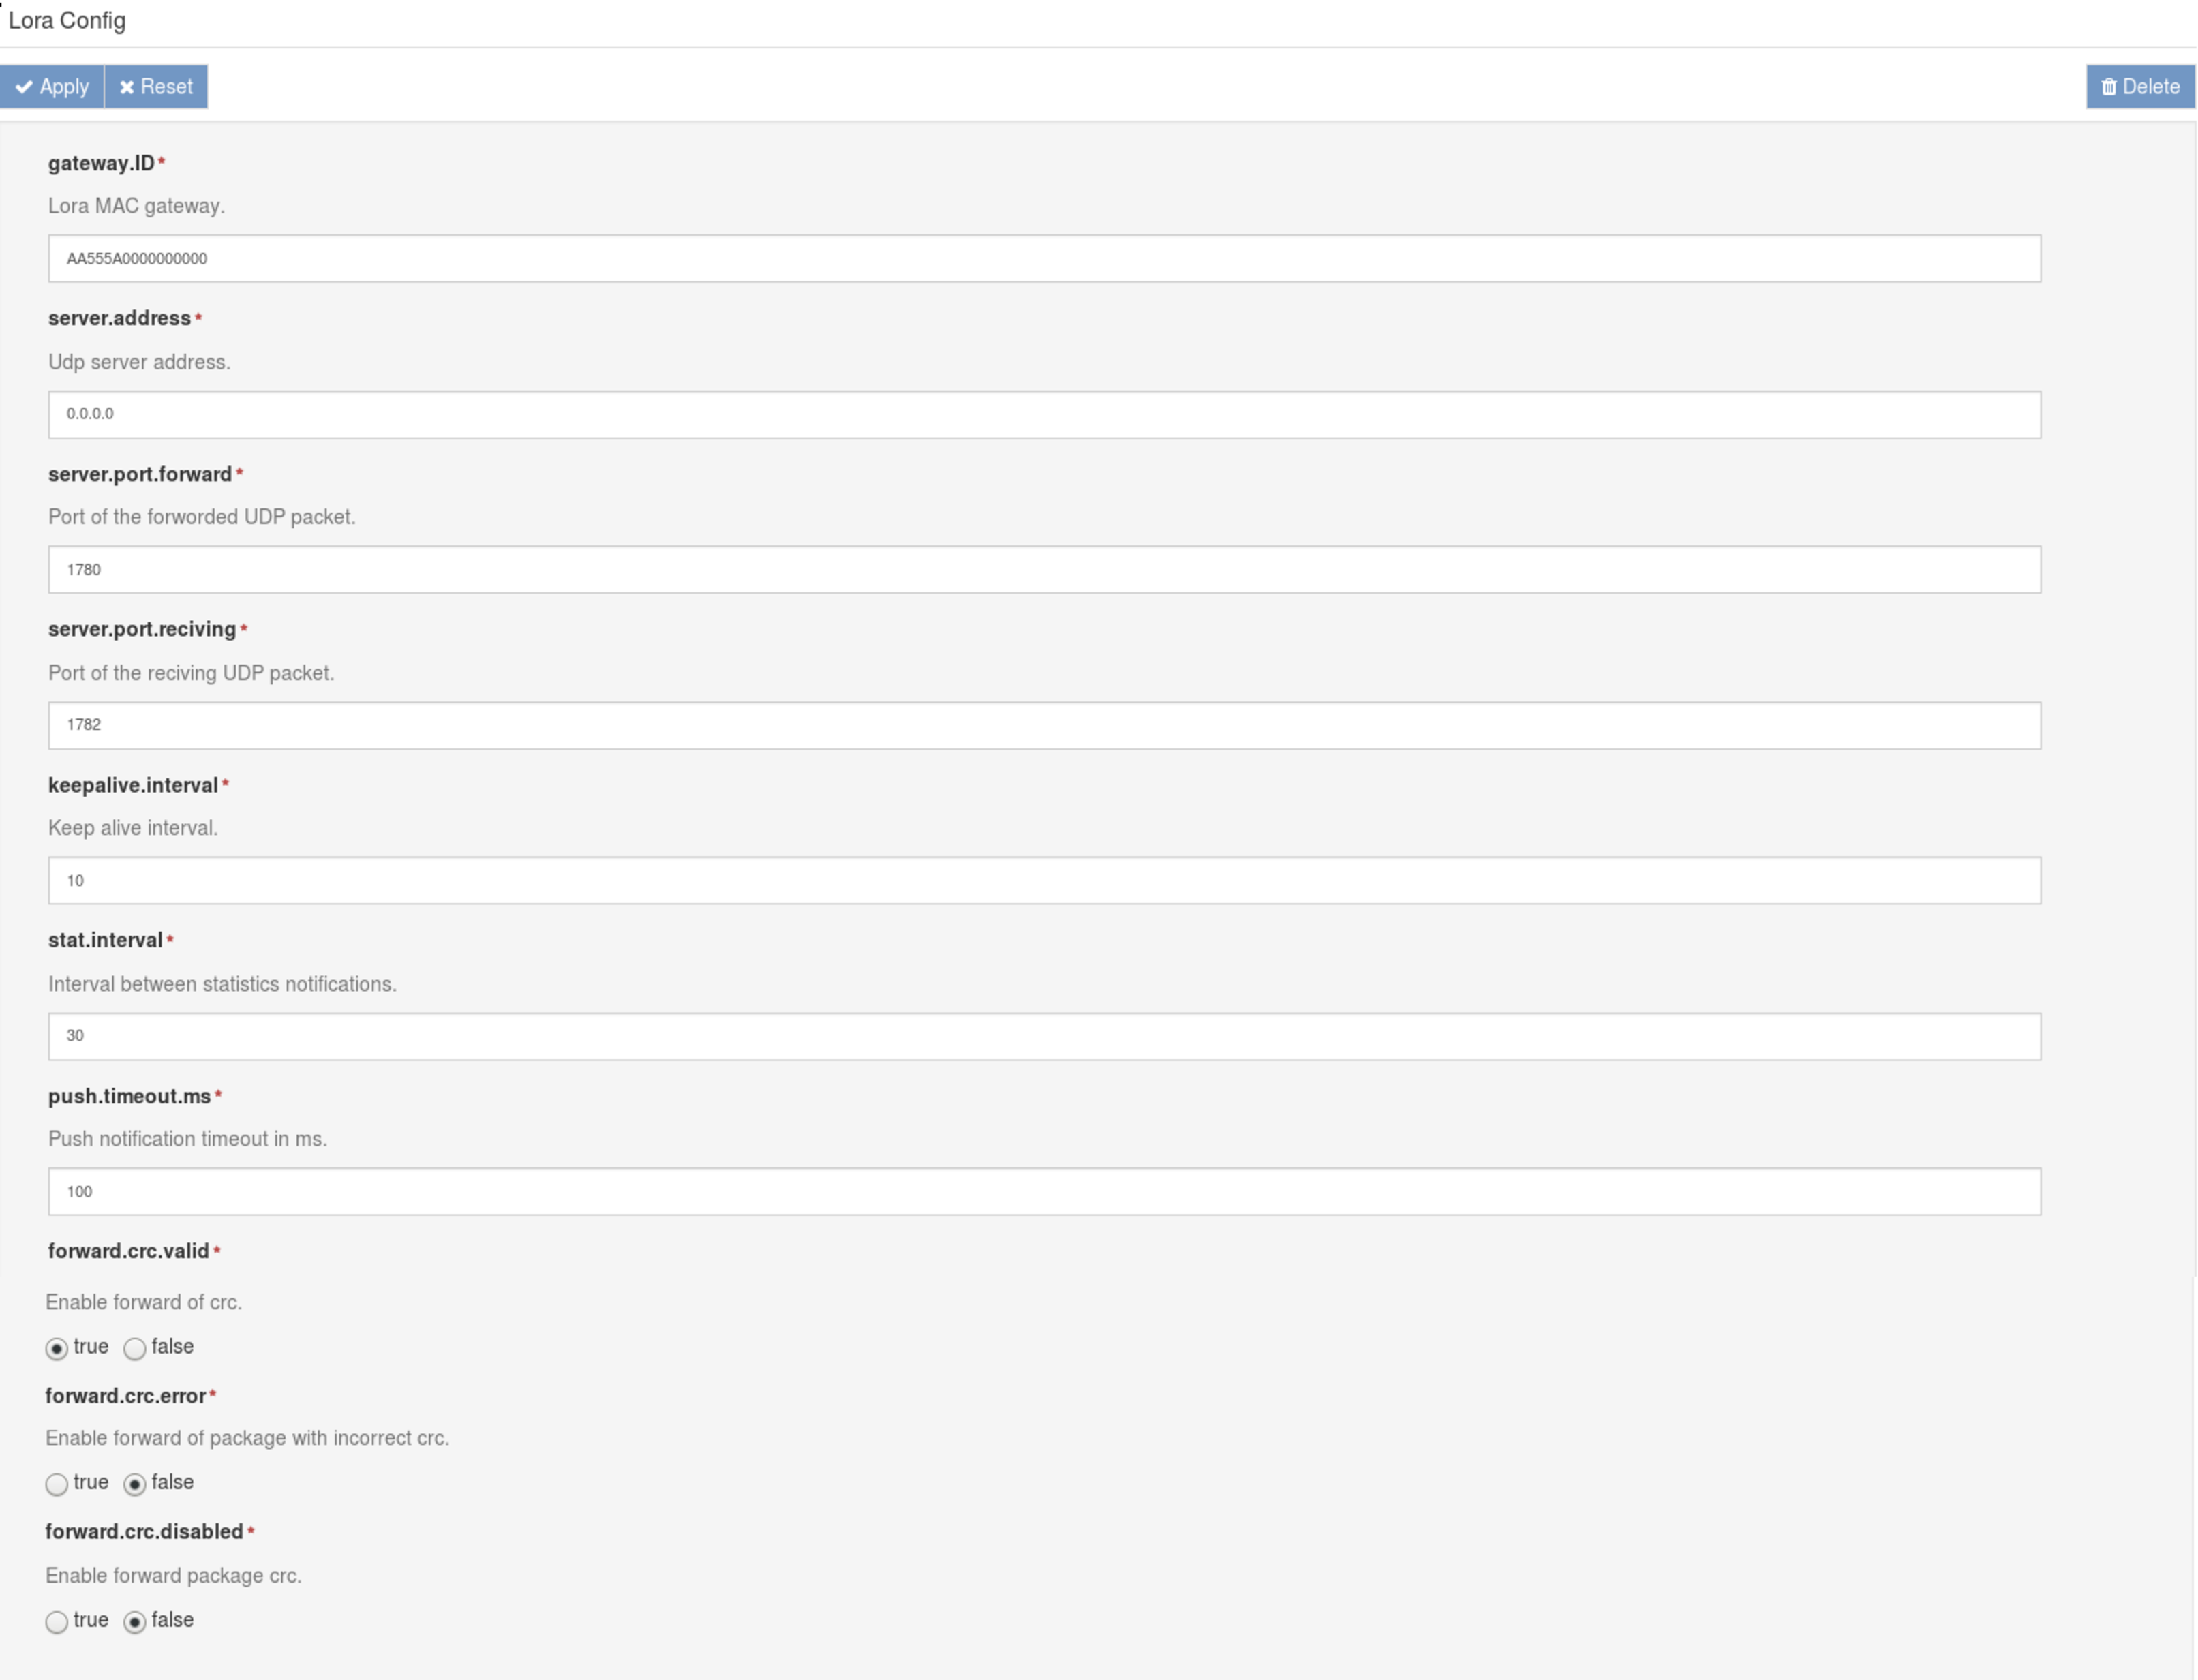
\includegraphics[width=16cm]{Lora_Config}
\caption{Architettura del software}
\label{fig:Software_stack}
\end{figure}



\subsection{Mqtt Bridge Config}
Il secondo bundle creato ha lo scopo di esporre all'utente un facile modo per
configurare  \emph{Lora Gateway Bridge}.  Anche in questo caso è necessario il
riavvio del applicativo per fare in modo che le modifiche abbiano effetto, anche
in questo caso è stata usata la libreria
\mint{Java}|import com.apache.commons.exec|
Tramite questo bundle l'utente finale ha la possibilità di decidere 
\begin{itemize}
\item il topic sul quale pubblicare i messaggi ricevuti in formato UDP dal
\emph{pkt forwarder}.
\item il topic al quale rimanere in ascolto .
\item su quale indirizzo e porta mandare/ricevere i pacchetti UDP.
\item a quale broker Mqtt iscriversi.
\item l'username e password per connettersi al broker.
\end{itemize}

\begin{figure}[h]
\centering 
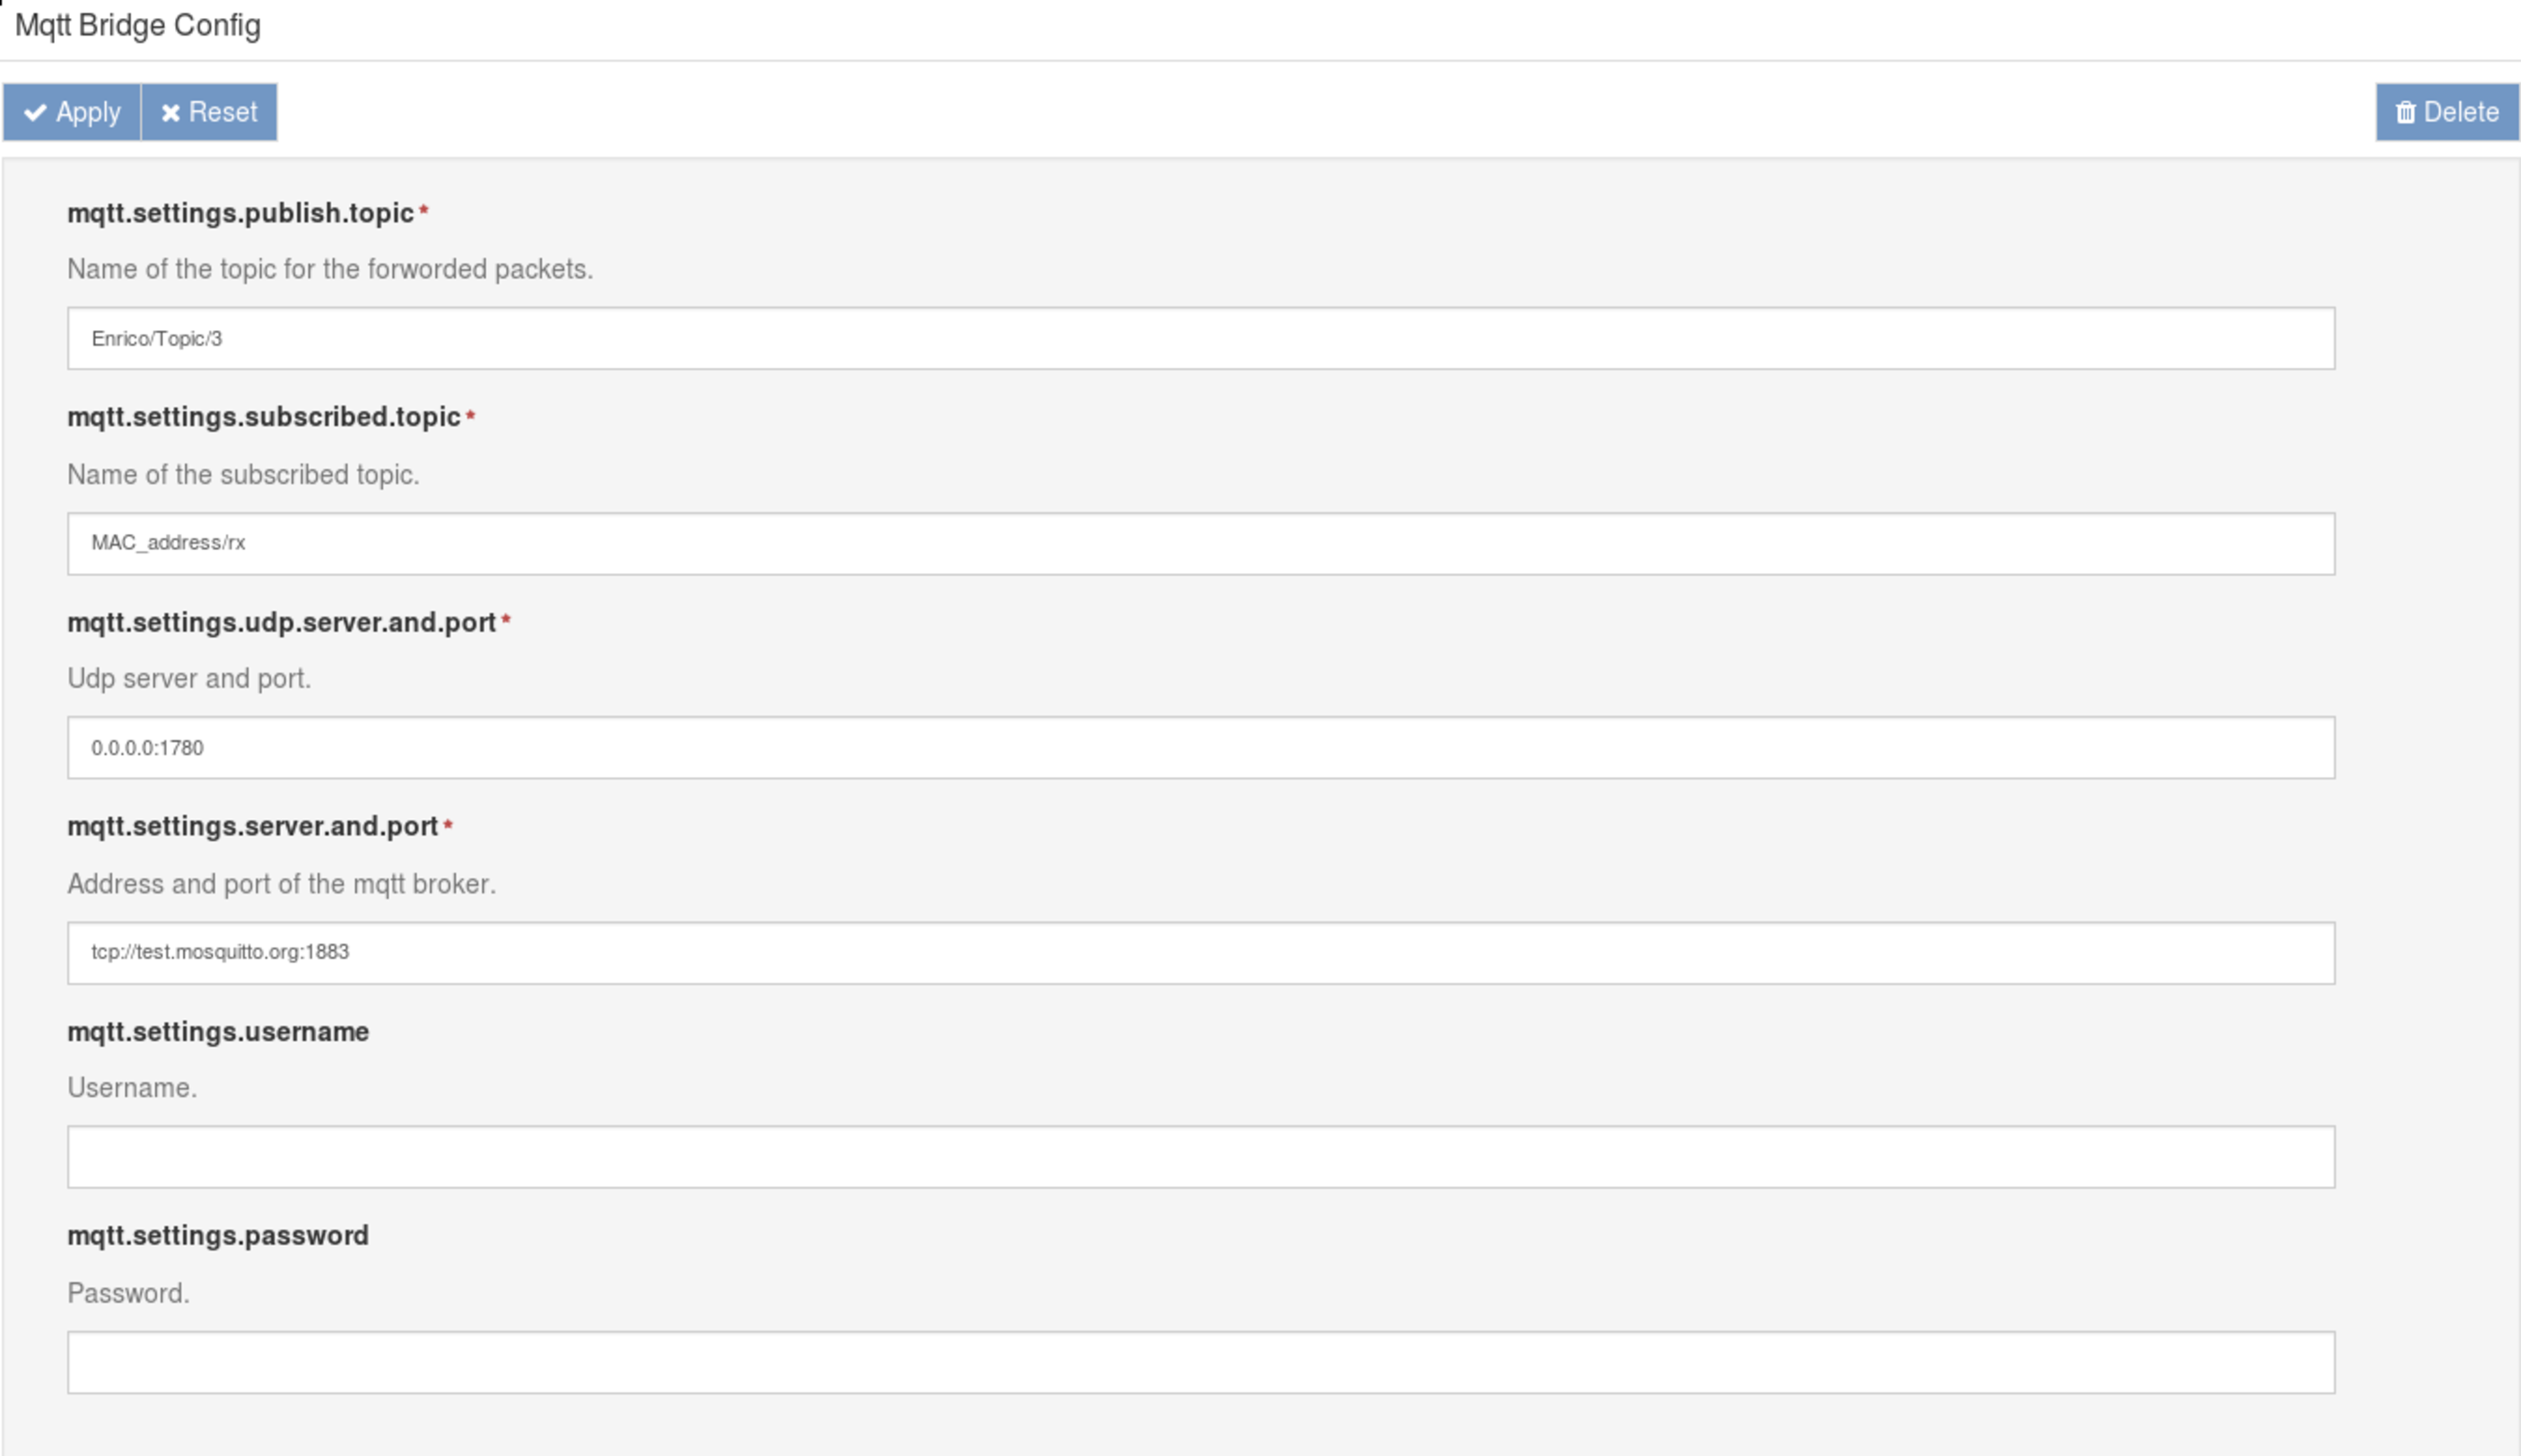
\includegraphics[width=16cm]{Mqtt_Bridge_Config}
\caption{Architettura del software}
\label{fig:Software_stack}
\end{figure}

\subsection{Misurazioni}
In via sperimentale, è stato scelto di installare in  il gateway
ReliaGate 10-11 ad una altezza di 11m. Configurato il gateway per l'utilizzo del
broker open source  mosquitto.org. La prova di ricezione è stata condotta per
tentativi, cercando di testare la massima distanza di trasmissione del
dispositivo LoRa Mote . 

\begin{figure}[h]
\centering 
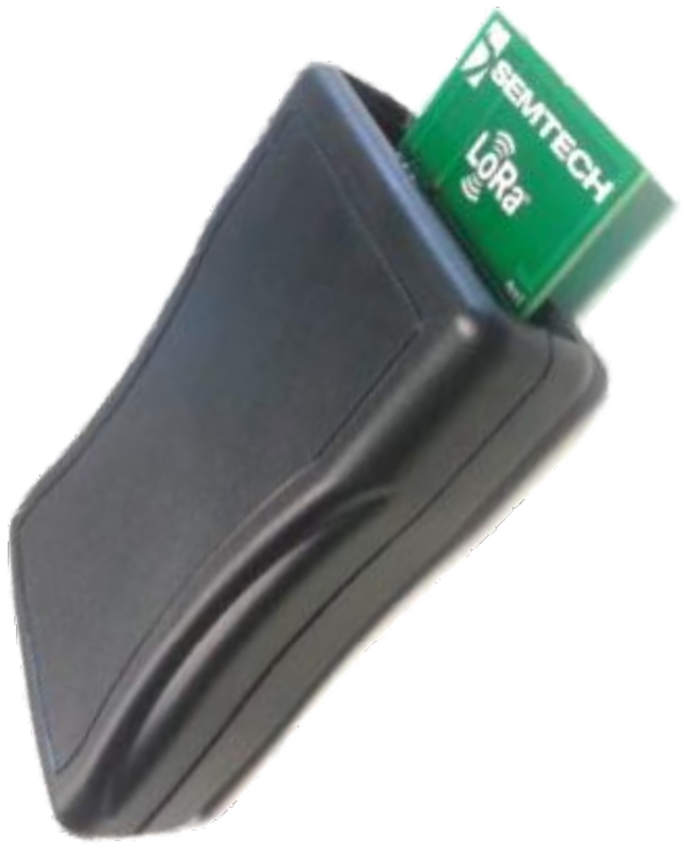
\includegraphics[width=4cm]{LoRaMote_no_wave}
\caption{Architettura del software}
\label{fig:Software_stack}
\end{figure}

Per constatare l'avvenuta ricezione del
messaggio è stata utilizzata l'applicazione Android gratuita MyMQTT, tramite la
quale è  possibile iscriversi ad un topic predefinito ed rimanere in ascolto dei
messaggi pubblicati in esso. 

\begin{figure}[h]
\centering 
\includegraphics[width=16cm]{map}
\caption{Copertura Lora}
\label{fig:map}
\end{figure}

\subsection{Osservazioni}
Come è facile ossevare dalla mappa in figura \ref{fig:map}, la distanza
massima raggiunta varia molto a seconda della conformazione del territorio. In
assenza di edifici in linea d'aria,  punto 8 nella figura \ref{fig:map}, è stato
possibili inviare un pachetto lora ad una distanza di 8.2[km]. Nelle effettuare
la prova è stato scelto di inviare al server Mqtt solo i pachetti ricevuti
correttamente riga \ref{line:crc_valid}
\begin{lstlisting}[
    language=json,escapechar=|] %language and your escape char
    "gateway_conf": {
        "gateway_ID": "AA555A0000000000",
        "server_address": "0.0.0.0",
        "serv_port_up": 1703,
        "serv_port_down": 1702,
        "keepalive_interval": 10,
        "stat_interval": 30,
        "push_timeout_ms": 100,
        "forward_crc_disabled": false,
        "forward_crc_valid": true, 
        "forward_crc_error": false |$\label{line:crc_valid}$|
    }
\end{lstlisting}



\subsection{Chip interno}
Per quanto riguarda la struttura interna dei moduli radio, non si hanno molte
informazioni dato che la tecnologia è proprietaria di Semtech. Nella
documentazione ufficiale è presente una rappresentazione grafica dei vari
blocchi presenti al interno dei moduli radio.

\begin{figure}[h]
\centering 
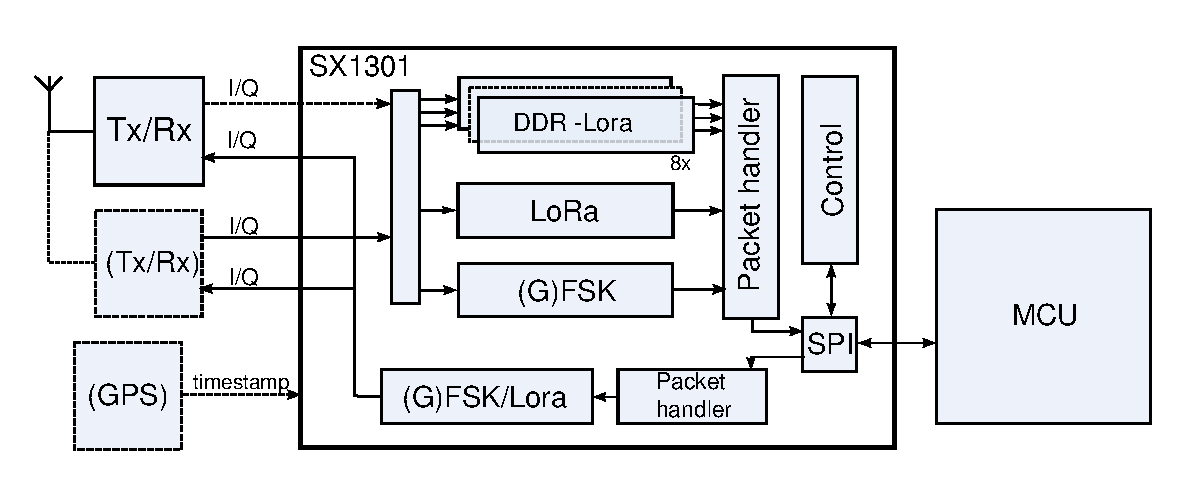
\includegraphics[width=11cm]{SX1301}
\caption{Struttura interna ricevitore SX1301}
\label{fig:sx1301}
\end{figure}

Dalla figura \ref{fig:sx1301} e dalla documentazione \improvement{inserire link}
che il gateway rimane in ascolto su 8 
canali diverse, le quali permettono di coprire tutti i vari SF. 
Questo è possibili data la quasi ortogonalità degli Spreading Factor
, in questo modo il ricevitore è in grado di ricevere un pacchetto
con uno Spreading Factor $i$ anche nel caso in cui si sovrapponga ad un altro
pacchetto con Spreading Factor pari a $j$, fintanto che $i\neq j$. Questa
pseudo-ortogonalità utilizzata in LoRa, permette di utilizzare differenti SF per
ottenere un maggiore throughput rispetto a schemi di modulazione tradizionale.
Il ricevitore  SX1301 può demodulare fino ad un massimo di 8 pacchetti
contemporaneamente, questo non vuol dire che ricevitori futuri non possano
demodulare contemporaneamente un numero di pacchetti maggiore.
Oltre a ciò grazie alla modulazione utilizzata abbiamo vantaggi quali:
\begin{itemize}
\item I vari nodi della rete, possono cambiare frequenza in ogni trasmissione in
modo casuale, andando a migliorare di molto la robustezza del sistema alle varie
interferenze.
\item Non è necessario avere tabelle contenenti informazioni riguardanti il
data-rate dei vari nodi. Ogni data-rate viene demodulato contemporaneamente.
\item È possibilie utilizzare più antenne nel gateway per realizzare il
cosidetto true antenna diversity, per aumentare la robustezza al multi-path
\end{itemize}
\unsure{Riguardare ultimo punto della documentazione pagina 14}

